\documentclass[11pt]{article}

\usepackage[a4paper,margin=1in]{geometry}
\usepackage[T1]{fontenc}
\usepackage{lmodern}
\usepackage{amsmath,amssymb,amsthm}
\usepackage{booktabs}
\usepackage{microtype}
\usepackage[hidelinks]{hyperref}
\usepackage{tikz}
\usetikzlibrary{arrows.meta,positioning}

\newtheorem{proposition}{Proposition}
\newtheorem{lemma}{Lemma}
\theoremstyle{remark}
\newtheorem{remark}{Remark}

\newcommand{\fl}[1]{\left\lfloor #1 \right\rfloor}
\newcommand{\cl}[1]{\left\lceil #1 \right\rceil}
\newcommand{\BPS}{10^{4}}
\newcommand{\NAV}{E}
\newcommand{\Lev}{\ell}
\newcommand{\bps}{\,\mathrm{bps}}
\newcommand{\dd}{\mathrm{d}}

\title{\textbf{Moor: Constant-Leverage Fund Shares\\ with Autonomous Rebalancing on Solana}}
\author{Moor Contributors}
\date{\today}

\begin{document}

\maketitle

\begin{abstract}
\noindent
We present Moor, a protocol for issuing fungible fund shares that track a constant target leverage on an underlying asset. Each fund is backed by a single collateralized debt position---a Kamino Lending ``Multiply'' obligation---owned by a program-derived vault. Share holders hold a pro-rata claim on the fund's net asset value (NAV), computed from oracle-priced collateral and debt; share issuance and redemption always use program-derived amounts, never caller-declared ones. Shares mint and redeem at NAV with fees paid in shares to a treasury, which leaves NAV per share unchanged up to integer rounding. Leverage is held inside a band by a permissionless controller with three modes---Routine, Ripcord, and WindDown---that derives the mode, trade size, slippage allowance, and post-trade bounds from on-chain state; the caller only routes a top-level flash loan and one decentralized-exchange swap. We formalize the NAV and share accounting, prove the NAV-per-share invariance of fees, derive the rebalancing sizing formulas and their fund-favoring rounding directions, and quantify the NAV cost of rebalancing and the inherent volatility drag of constant leverage. Every flow executes as a single atomic transaction with same-slot oracle freshness and flash-loan binding.
\end{abstract}

\section{Introduction}

On-chain leveraged exposure is typically obtained through per-user debt: perpetual futures, margin accounts, or individual lending positions. Each user must monitor a health factor, post additional margin, and carries individual liquidation risk. The resulting positions are operationally expensive and socially inefficient: they fragment liquidity, require per-user risk engines, and expose every holder to idiosyncratic liquidation events.

Moor replaces per-user leverage with a \emph{fund-level} instrument. A Moor fund issues an SPL share token that represents a pro-rata claim on a single leveraged position, a Kamino Lending obligation that holds collateral $D$ and debt $B$. The fund targets a fixed leverage multiple (e.g., $2\times$ or $3\times$) and continuously corrects deviations through a permissionless rebalancing controller. Because the obligation is owned by the fund's vault and not by any user, holders never face margin calls, health-factor monitoring, or individual liquidation: the worst case is a decline in NAV per share, shared pro rata. In exchange for this convenience, the fund structure introduces three problems that this paper formalizes and solves: (i) correct share accounting at a NAV that is only observable through an oracle, (ii) a rebalancing policy that restores target leverage without trusting the party who executes it, and (iii) an execution model that makes every operation atomic with respect to price and debt state.

\paragraph{Contributions.}
\begin{enumerate}
\item \textbf{NAV and share model.} We define NAV as the oracle-priced difference between the obligation's collateral and debt, define leverage and the dust/underwater regime, and specify mint and redemption as proportional operations with a single truncation (\S\ref{sec:nav}).
\item \textbf{Fee neutrality.} We prove that mint, redeem, and streaming fees, when paid in shares to a treasury, leave NAV per share unchanged in exact arithmetic and move it by at most integer rounding dust; truncations are directed to favor the fund's remaining holders (\S\ref{sec:invariants}).
\item \textbf{Redemption capacity.} We derive a closed-form, integer-only cap on the shares that a reserve's current spot liquidity can serve, which implements partial fills without a withdrawal queue (\S\ref{sec:servable}).
\item \textbf{Rebalancing controller.} We specify a band controller with three modes---Routine, Ripcord, and WindDown---whose target, trade value, slippage, bounty, and acceptance bounds are all derived on-chain; we give the exact rounding directions and the resulting NAV cost (\S\ref{sec:rebalance}).
\item \textbf{Atomic execution.} We describe the single-transaction envelope that binds each flow to a verified flash loan, a same-slot oracle refresh, and an ordered session, which removes the class of stale-price and partial-execution failures (\S\ref{sec:security}).
\end{enumerate}

The reference implementation is a Solana program, unit-tested on the host and
integration-tested against a forked Kamino mainnet market.

\noindent
Its program id is
{\small\texttt{4vfgiGbN4Je9m5\allowbreak DCb4NnFmF7W2N7\allowbreak aHBu74HpL8QXzKko}}.

\section{System Model}
\label{sec:model}

\subsection{Kamino obligations}

Kamino Lending (\texttt{klend}) is an over-collateralized lending protocol. Liquidity providers supply a \emph{reserve} and receive cTokens representing their claim; borrowers open \emph{obligations}, each a collateralized debt position identified by the tuple (lending market, owner, collateral mint, debt mint). An obligation stores one deposit slot (cToken collateral) and one borrow slot (native debt). Prices are written by Scope oracles during a refresh and carry a per-slot freshness marker. A \emph{Multiply} obligation is an obligation whose debt was borrowed against its own collateral; Moor uses exactly one such obligation per fund, so the obligation holds a single deposit slot and a single borrow slot.

Let $D$ denote the USD market value of the obligation's deposit slot and $B$
that of its borrow slot. Both are refreshed at Scope oracle prices and stored
as scaled fixed-point numbers with $2^{60}$ fractional resolution. Moor never
re-derives Kamino's internal math; it reads these two values and treats their
difference as the fund's equity.

\subsection{Fund and share token}

A fund is a program-derived address keyed by the tuple (underlying mint, debt mint, target leverage). The same asset pair at two targets therefore yields two independent funds with independent obligations. The fund records immutable identity (mints, reserves, lending market, obligation, flash-loan source, treasury), configuration (bands, fees, caps, cooldowns), and live accounting (share supply $n$, streaming-fee clock, display fields).

A separate \emph{vault} PDA, derived from the fund, is the owner of the Kamino obligation and the token authority of the fund's transit token accounts. It is a zero-data system account: it exists only to sign Kamino CPIs and to own the position. Share holders therefore hold a claim on a single blended position; there is no per-user obligation and no credit delegation.

The fund mints an SPL share token with six decimals. The share supply $n$ is measured in base units, so one whole share equals $10^{6}$ base units. All share math below is in base units.

\subsection{Lifecycle}

A fund is created in the \textsc{Active} state and can move exactly once to \textsc{Closing}, by the admin. The distinction is not cosmetic:

\begin{center}
\small
\begin{tabular}{@{}lll@{}}
\toprule
 & \textsc{Active} & \textsc{Closing} \\
\midrule
Bootstrap / mint & allowed (unless paused) & rejected \\
Redeem & allowed, fee charged & while debt $>0$, fee waived \\
Streaming fee & accrues & frozen at zero \\
Rebalance & Routine / Ripcord & WindDown / Ripcord to $1.0\times$ \\
Exit & --- & pro-rata exits once debt $=0$ \\
\bottomrule
\end{tabular}
\end{center}

Closing is one-way. It exists so that a fund can be retired without forcing a market sale: debt is first repaid to zero by the wind-down crank, after which the remaining collateral is a pro-rata claim that no longer needs an oracle price.

\subsection{Atomic execution}
\label{sec:envelope}

Every flow---bootstrap, mint, redeem, and rebalance---is a \emph{single transaction} with the shape
\[
\texttt{begin} \;\rightarrow\; \texttt{step} \;\rightarrow\; \texttt{step} \;\rightarrow\; \texttt{finalize}.
\]
The client composes the top-level Kamino flash loan and one DEX swap; Moor's program only issues the vault-signed deposit, borrow, repay, and withdraw legs. This division is forced by Kamino: flash loans must be top-level instructions (Kamino rejects them via CPI), and the vault PDA cannot sign a top-level instruction. Figure~\ref{fig:arch} shows the account relationships; Figure~\ref{fig:envelope} shows a representative envelope.

\begin{figure}[t]
\centering
\resizebox{\textwidth}{!}{%
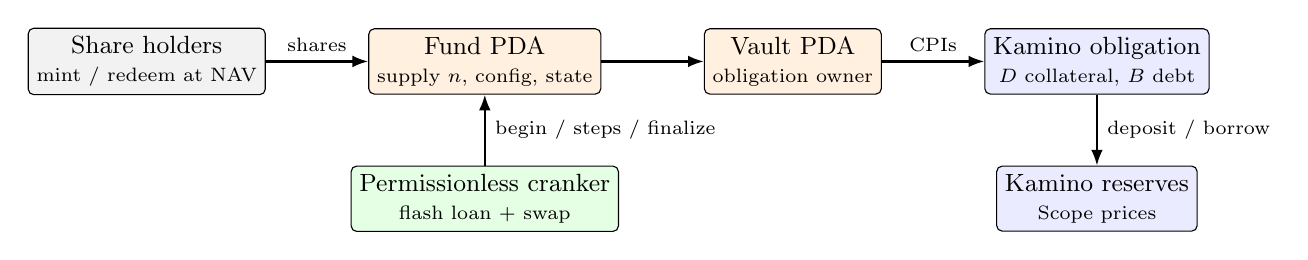
\begin{tikzpicture}[
  font=\small,
  box/.style={draw, rounded corners=2pt, align=center, inner sep=3pt, minimum height=8mm},
  arr/.style={-{Latex[length=2mm]}, thick},
  node distance=9mm and 13mm
]
\node[box, fill=black!5] (holders) {Share holders\\[-1pt]\scriptsize mint / redeem at NAV};
\node[box, fill=orange!12, right=of holders] (fund) {Fund PDA\\[-1pt]\scriptsize supply $n$, config, state};
\node[box, fill=orange!12, right=of fund] (vault) {Vault PDA\\[-1pt]\scriptsize obligation owner};
\node[box, fill=blue!8, right=of vault] (oblig) {Kamino obligation\\[-1pt]\scriptsize $D$ collateral, $B$ debt};
\node[box, fill=blue!8, below=of oblig] (reserves) {Kamino reserves\\[-1pt]\scriptsize Scope prices};
\node[box, fill=green!10, below=of fund] (cranker) {Permissionless cranker\\[-1pt]\scriptsize flash loan + swap};
\draw[arr] (holders) -- node[above,font=\scriptsize]{shares} (fund);
\draw[arr] (fund) -- (vault);
\draw[arr] (vault) -- node[above,font=\scriptsize]{CPIs} (oblig);
\draw[arr] (oblig) -- node[right,font=\scriptsize]{deposit / borrow} (reserves);
\draw[arr] (cranker) -- node[right,font=\scriptsize]{begin / steps / finalize} (fund);
\end{tikzpicture}%
}
\caption{A fund owns one Kamino obligation through a vault PDA. Share holders interact with the fund at NAV; anyone may crank a rebalance, supplying a flash loan and a swap, while the program fixes every trade amount.}
\label{fig:arch}
\end{figure}

\begin{figure}[t]
\centering
{\small
\begin{verbatim}
[cu]                        compute budget
flash_borrow                klend, top level
refresh set                 klend, top level
mint_begin                  Moor: checks, snapshot, session init
swap (debt -> collateral)   client, output into vault ATA
mint_deposit_step           Moor: vault-signed klend deposit
refresh set                 klend, top level
mint_borrow_step            Moor: vault-signed klend borrow
flash_repay                 klend, top level
refresh set                 klend, top level
mint_finalize               Moor: NAV read, share issuance, session close
\end{verbatim}
}
\caption{The mint envelope. Every flow has the same shape: the flash pair brackets the transaction, and the session opened by \texttt{begin} is closed by \texttt{finalize} in the same transaction.}
\label{fig:envelope}
\end{figure}

Three mechanisms make the envelope safe:

\begin{itemize}
\item \textbf{Finalize binding.} Every \texttt{begin} scans the instructions sysvar for a later Moor instruction carrying the same flow's \texttt{finalize} discriminator and both the fund and the session account. If none exists the instruction reverts. Because \texttt{finalize} closes the session, a session can never outlive its transaction and a half-built envelope can never land.
\item \textbf{Session ordering.} A session stores a step bitmap (\textsc{begin}, \textsc{first}, \textsc{second}) and the caller's key. Each obligation-operation step requires its bit and sets it, so steps run exactly once, in order; a reordered, repeated, or missing step reverts. All amounts are computed once in \texttt{begin} and replayed by the steps, so a caller cannot skew the proportion.
\item \textbf{Fresh state.} Every Moor read of an obligation or reserve requires a same-slot refresh: the account must be owned by Kamino, its last-update slot must equal the current slot, its stale flag must be clear, and---when a price is used---its price status must be fully valid. A read without a same-slot refresh reverts. The flashed amount is read from the preceding top-level flash-borrow instruction's data, never from a caller argument, and the matching flash-repay must sit at the caller-declared instruction index.
\end{itemize}

\section{NAV and Share Accounting}
\label{sec:nav}

\subsection{NAV, leverage, and the dust regime}

The fund's net asset value is
\begin{equation}
\NAV = D - B,
\label{eq:nav}
\end{equation}
where $D$ and $B$ are the refreshed USD market values of the obligation's deposit and borrow slots. If $B > D$ the fund is \emph{underwater} and no NAV exists; mint and redeem are rejected, while risk-reducing rebalancing remains available. Leverage in basis points is
\begin{equation}
\Lev = \frac{\BPS\,D}{\NAV},
\label{eq:leverage}
\end{equation}
and we adopt the convention
\begin{equation}
\Lev = \infty \quad\text{(represented as \texttt{u32::MAX})}
\qquad\text{when } \NAV \le \delta \ \text{or } B > D,
\end{equation}
with dust floor $\delta = 1/1000$ USD. Reading infinite leverage as ``past every threshold'' keeps risk logic live: a dust-sized or underwater fund always selects the Ripcord mode and cannot satisfy any leverage ceiling. Because a leverage ceiling check is of the form $\Lev < \Theta$, the sentinel fails closed rather than open.

\subsection{Minting}

A mint deposits collateral and borrows against it in the same transaction, so the fund's realized NAV grows by
\[
\Delta\NAV = \NAV_{\mathrm{after}} - \NAV_{\mathrm{before}} > 0.
\]
Shares are issued against \emph{realized} NAV growth, never against the declared deposit. This is the anti-theft invariant: a caller cannot overstate the value they contributed, because the value is measured from the obligation before and after the envelope. With share supply $n$ and mint fee $\phi_m$ in basis points, the gross issuance is
\begin{equation}
g = \fl{\frac{\Delta\NAV \cdot n}{\NAV}},
\qquad
g_{\mathrm{fee}} = \fl{\frac{g\,\phi_m}{\BPS}},
\qquad
n' = n + g,
\label{eq:mint}
\end{equation}
where $g - g_{\mathrm{fee}}$ goes to the depositor and $g_{\mathrm{fee}}$ to the treasury. The supply grows by the full gross $g$; the fee is a transfer of claims between the depositor and the treasury, not a change in value per share. We compute $g$ by cross-multiplication with a single truncation at the end, never by forming a per-share intermediate, which bounds the rounding error to one unit of the final quantity.

\paragraph{Blended-leverage check.}
Mint levers only the marginal equity at target. If the fund entered at deposited value $D_0$ and the depositor added $\Delta\NAV$ of equity, the expected post-state deposited value is $D_0 + \Delta\NAV \cdot T/\BPS$ where $T$ is the target in basis points. \texttt{mint\_finalize} therefore checks
\begin{equation}
\left| \Lev_{\mathrm{after}} - \frac{\BPS\bigl(D_0 + \Delta\NAV \cdot T/\BPS\bigr)}{\NAV_{\mathrm{after}}} \right| \le \tau
\quad\text{and}\quad
\Lev_{\mathrm{after}} < \Theta,
\label{eq:blended}
\end{equation}
where $\tau$ is the leverage tolerance and $\Theta$ the ripcord threshold. The slack absorbs swap slippage and the Kamino borrow fee. This check is what prevents a minter from depositing at a leverage materially different from the fund's target and diluting the blend.

\subsection{Bootstrap}

The first deposit establishes NAV from nothing, so there is no $\NAV_{\mathrm{before}}$. Moor fixes the initial price at \$1 per whole share:
\begin{equation}
n = \fl{10^{6}\,\NAV},
\label{eq:bootstrap}
\end{equation}
i.e.\ the NAV in USD with six decimals. Of these, $1000$ base units are minted to a dead account whose authority is the vault (never spendable) and the remainder to the depositor. The instruction requires $n > 1000$, so supply can never return to zero and no later flow can be priced against an empty denominator. Bootstrap also requires post-state leverage within $\tau$ of target and below $\Theta$.

\subsection{Redemption}

A redemption of $s$ shares is the mirror image. Let $s_{\max}$ be the servable cap of \S\ref{sec:servable}. The fund serves
\begin{equation}
a = \min(s, s_{\max}),
\qquad
a_{\mathrm{fee}} = \fl{\frac{a\,\phi_r}{\BPS}},
\qquad
u = a - a_{\mathrm{fee}},
\qquad
f = \frac{u}{n},
\label{eq:redeem}
\end{equation}
where $a_{\mathrm{fee}}$ is transferred to the treasury, $u$ is burned, and $f$ is the fraction of the fund unwound. The debt and collateral legs are proportional:
\begin{equation}
R = \fl{\beta f},
\qquad
C = \fl{c f},
\qquad
n' = n - u,
\label{eq:redeem-legs}
\end{equation}
with $\beta$ the obligation's native debt (scaled-fixed-point bits) and $c$ its deposited cTokens. The repay step repays $R$ and returns any unused flash margin to the caller; the withdraw step withdraws $C$ and records the measured underlying proceeds; \texttt{finalize} pays exactly the recorded amount. An optional swap after \texttt{finalize} converts the paid-out collateral into the debt token before the flash is settled, so a redeemer need not hold or front any debt tokens.

Two properties matter. First, only the net $u$ is burned and unwound: the fee shares remain outstanding at the treasury. Second, the redeemer is paid exactly the collateral their own withdrawal freed, not the vault's balance. The latter closes a cross-user race in which one redeemer's finalize could consume collateral freed by another.

\subsection{Redemption capacity and partial fills}
\label{sec:servable}

A solvent fund can still be illiquid: its collateral sits in a reserve whose spot available liquidity may be less than the value being withdrawn. Rather than queue withdrawals, Moor caps each redemption at the shares the reserve can serve right now, and leaves the unserved remainder with the holder, who can retry later. The cap inverts the cToken exchange rate. Let $A$ be the reserve's available liquidity, $\beta_r$ its borrowed amount, and $S_c$ its cToken supply. A withdrawal of $w$ cTokens redeems $w \cdot (A + \beta_r)/S_c$ underlying, so the cToken amount the reserve can serve is
\begin{equation}
w_{\max} = \kappa(A) = \fl{\frac{A\,S_c}{A + \cl{\beta_r}}},
\label{eq:ctoken-rate}
\end{equation}
where the borrowed amount is rounded up so the estimate never exceeds what Kamino would allow. Inverting the proportional withdrawal of \eqref{eq:redeem-legs} and grossing the fee back up gives
\begin{equation}
s_{\max} = \fl{\frac{\fl{\kappa(A)\,n / c}\;\BPS}{\BPS - \phi_r}},
\qquad
\text{with } s_{\max} = 0 \text{ if } c=0,\ n=0,\ \text{or } \phi_r = \BPS.
\label{eq:servable}
\end{equation}
Every division rounds down and the borrowed term rounds up, so $s_{\max}$ is conservative with respect to the fund. The cap deliberately excludes DEX depth: a redeemer who wants more can swap separately, and the cap's purpose is to keep the redemption itself solvent. All quantities are computed in $128$-bit integers; a mainnet-sized reserve makes the product $A \cdot S_c$ large enough to overflow fixed-point representations, so this computation is deliberately kept in integer arithmetic.

\subsection{Streaming fee}

A time-based management fee accrues lazily whenever a user flow touches the fund. With streaming rate $\phi_s$ in basis points per year and elapsed wall-clock time $\Delta t$ seconds,
\begin{equation}
\Delta n_s = \fl{\frac{n\,\phi_s\,\Delta t}{365.25 \cdot 86400 \cdot \BPS}},
\label{eq:streaming}
\end{equation}
minted to the treasury. Accrual runs \emph{before} the user's own share math, so a user never pays for or benefits from a period they were not present; \emph{before} a configuration change, so a rate change is never retroactive; and \emph{before} closing, at the active rate, after which the rate is frozen to zero. Rebalancing does not accrue; the next mint or redeem settles the whole gap. Because supply grows while NAV does not, the streaming fee makes NAV per share decay at the annual rate $\phi_s$---a deliberate, monotone dilution of all holders in favor of the treasury.

\subsection{Invariants}
\label{sec:invariants}

\begin{proposition}[Mint preserves NAV per share]
In exact arithmetic, a mint according to \eqref{eq:mint} leaves NAV per share unchanged; with truncation, it can only increase NAV per share for existing holders.
\end{proposition}
\begin{proof}
Let $g = \Delta\NAV \cdot n/\NAV$ exactly. Then
$\NAV' = \NAV + \Delta\NAV$ and $n' = n + g = n\,(1 + \Delta\NAV/\NAV) = n\,\NAV'/\NAV$,
so $\NAV'/n' = \NAV/n$. The implementation truncates $g$ down, so $g \le \Delta\NAV\,n/\NAV$ and hence $n' \le n\,\NAV'/\NAV$, which gives $\NAV'/n' \ge \NAV/n$. The split of $g$ between depositor and treasury is irrelevant: both are claims on the same enlarged pool.
\end{proof}

\begin{proposition}[Redemption preserves NAV per share]
In exact arithmetic, a redemption according to \eqref{eq:redeem}--\eqref{eq:redeem-legs} leaves NAV per share unchanged; with truncation, the change is bounded by integer rounding dust.
\end{proposition}
\begin{proof}
Removing fraction $f$ of every deposit and borrow slot removes $fD$ of collateral value and $fB$ of debt value, hence $f(D-B) = f\NAV$ of NAV, while retiring $u = fn$ shares. Therefore $\NAV'/n' = \NAV(1-f)/(n(1-f)) = \NAV/n$. The fee shares remain outstanding and are unaffected in value; the fee is a transfer from the redeemer to the treasury, not a dilution of remaining holders.
\end{proof}

\begin{lemma}[Rounding directions]
The implementation rounds toward the fund: mint issuance and redeem legs truncate down; a relever borrows less (floor) and demands more collateral in (ceil); a delever releases less collateral (the cToken amount is floored with the reserve's borrowed term rounded up); and a full-debt repay rounds up so that no dust debt remains.
\end{lemma}

The host test suite verifies \eqref{eq:mint}--\eqref{eq:redeem-legs} numerically: mint and redeem fees move NAV per share by at most one $10^{-6}$ USD unit, and the fee split is exactly $\fl{g\phi/\BPS}$.

\section{Rebalancing}
\label{sec:rebalance}

Leverage drifts with the underlying price: absent intervention, a fund at target $T$ that experiences a price move will see its leverage move in the opposite direction. Moor corrects drift through a permissionless controller. Nobody chooses the mode or the amounts: \texttt{rebalance\_begin} derives everything from the refreshed obligation, and the steps replay the derived amounts. The cranker supplies only the flash loan and the swap.

\subsection{Bands and mode selection}

Each fund defines a target $T$, a relever trigger $T_r < T$, a delever trigger $T_d > T$, and a ripcord danger threshold $\Theta > T_d$ (all in basis points). Given the refreshed leverage $\Lev$, the closing flag, and whether debt exists, the mode is selected deterministically:

\begin{center}
\begin{tabular}{@{}llll@{}}
\toprule
Condition & Mode & Direction & Target $L'$ \\
\midrule
Closing, debt $=0$ & --- (no-op) & --- & --- \\
Closing, $\Lev \ge \Theta$ & Ripcord & delever & $1.0\times$ \\
Closing, $\Lev < \Theta$ & WindDown & delever & $1.0\times$ \\
$\Lev \ge \Theta$ & Ripcord & delever & $T$ \\
$\Lev > T_d$ & Routine & delever & recentered \\
$\Lev < T_r$ & Routine & relever & recentered \\
otherwise & --- (no-op) & --- & --- \\
\bottomrule
\end{tabular}
\end{center}

The Ripcord mode is the risk-off path: it engages at $\Theta$, below the leverage at which Kamino would liquidate the position, and it is the only mode that pays a bounty. WindDown is the retirement path, used after the admin moves the fund to \textsc{Closing}; it always targets $1.0\times$ so that the debt can be driven to zero and holders can exit pro rata.

\subsection{Recentering}

A Routine rebalance does not jump to the target; it moves part of the way, with recentering speed $RS$ in basis points:
\begin{equation}
L' = \fl{\frac{T(\BPS - RS) + \Lev\,RS}{\BPS}},
\qquad RS \in [0,\BPS).
\label{eq:recenter}
\end{equation}
At $RS = 0$ the fund returns exactly to target; as $RS$ grows, the controller corrects only the excess beyond a moving fraction of the gap. This is a proportional controller on leverage whose gain $RS$ can be tuned against fee and cost data. Note that $L'$ is defined only when $\Lev$ is finite, which is guaranteed for Routine by $\Lev < \Theta$.

\subsection{Trade sizing}

The trade value $X$ is the USD value that must be exchanged to move leverage from $\Lev$ to $L'$. With $D$ and $B$ the refreshed market values, the required delever is
\begin{equation}
\mathrm{need} =
\begin{cases}
D - L'\,\NAV/\BPS, & \text{delever},\\[2pt]
L'\,\NAV/\BPS - D, & \text{relever},
\end{cases}
\qquad
X = \min\bigl(\mathrm{need},\ \nu(M; P_d, d_d)\bigr),
\label{eq:trade}
\end{equation}
where $M$ is the maximum trade size in debt-token native units, $P_d$ the debt price in USD per whole token, $d_d$ its mint decimals, and $\nu(v;P,d) = vP/10^{d}$ converts native units to USD. For a delever, $X$ is additionally capped at $B$, since repaying more than the outstanding debt is impossible. When the fund is underwater or at dust NAV, $\mathrm{need}$ is treated as unbounded and the caps bind: the controller repays as much debt as the trade-size cap allows. If $X = 0$ after capping, the transaction reverts as unnecessary.

\subsection{Delever amounts}

Let $s$ be the mode's maximum slippage in basis points, $\rho$ the ripcord reward rate, $C$ the absolute reward cap in debt-token native units, and $\beta$ the obligation's native debt. A delever repays
\begin{equation}
\text{repay} =
\begin{cases}
\cl{\beta}, & X \ge B,\\[2pt]
\fl{\nu^{-1}(X; P_d, d_d)}, & X < B,
\end{cases}
\label{eq:repay}
\end{equation}
where $\nu^{-1}(V;P,d) = V10^{d}/P$ converts USD to native. The full-debt case rounds up so that no dust debt survives. The collateral released to the cranker is
\begin{equation}
W = \frac{X\,\BPS}{\BPS - s} + \text{bounty},
\qquad
\text{bounty} = \min\!\left(\frac{X\rho}{\BPS},\ \nu(C; P_d, d_d)\right),
\label{eq:withdraw}
\end{equation}
with $\text{bounty} = 0$ except in Ripcord mode, and the cToken amount withdrawn is
\begin{equation}
\text{withdraw} = \min\bigl(\kappa\bigl(\fl{\nu^{-1}(W; P_c, d_c)}\bigr),\ c\bigr),
\label{eq:withdraw-ct}
\end{equation}
where $c$ is the obligation's cToken balance. Because $W = X/(1-s/10^4) + \text{bounty}$, the cranker repays $X$ of debt and receives collateral worth $X/(1-s/10^4)$ plus the bounty: the slippage allowance is exactly the spread between what the cranker pays and what it receives. The design fixes the trade price, so a rational cranker captures the full spread; the program therefore treats $s$ as an expected cost, not a worst case (see \S\ref{sec:cost}).

\subsection{Relever amounts}

A relever borrows against newly deposited collateral:
\begin{equation}
\text{borrow} = \fl{\nu^{-1}(X; P_d, d_d)},
\qquad
\text{min collateral in} = \cl{\nu^{-1}\bigl(X(1 - s/\BPS); P_c, d_c\bigr)}.
\label{eq:relever}
\end{equation}
The swap must deliver at least the minimum collateral into the vault; the deposit step reverts otherwise. The borrow is floored and the collateral requirement is ceiled, both in the fund's favor.

\subsection{Cooldowns, slippage, and bounty}

Each mode carries its own parameters, and each rebalance stamps a cooldown clock:

\begin{center}
\small
\begin{tabular}{@{}lllll@{}}
\toprule
Mode & Cooldown clock & Slippage $s$ & Bounty & Trigger \\
\midrule
Routine & \texttt{rebalance\_cooldown} & $\le 100$ bps & none & band breach \\
Ripcord & \texttt{twap\_cooldown} & $\le 1000$ bps & $\rho \le 200$ bps, cap $C$ & $\Lev \ge \Theta$ \\
WindDown & \texttt{twap\_cooldown} & $\le 100$ bps & none & closing, debt $>0$ \\
\bottomrule
\end{tabular}
\end{center}

The longer Ripcord cooldown is a rate limit on the risk-off path, sized to the price-oracle TWAP window so that repeated cranking cannot drain the fund through the slippage allowance. The bounty compensates the cranker for acting under stress. The hard caps on $s$ and $\rho$ bound the damage a compromised admin key could do through configuration, since the admin also controls the parameters that trigger the mode.

\subsection{Post-state bounds}
\label{sec:bounds}

After the steps, \texttt{rebalance\_finalize} re-reads leverage and accepts the trade only if
\begin{align}
\text{delever:}\quad
&(\Lev_{\mathrm{after}} < \Lev_{\mathrm{before}} \ \text{or}\ \Lev_{\mathrm{before}} = \infty)
&&\text{(improve or not worsen)}\notag\\
&\text{and } \Lev_{\mathrm{after}} + \tau \ge L' \ \text{for Routine/Ripcord}
&&\text{(no undershoot)}\notag\\
&\text{and } \Lev_{\mathrm{after}} < \Theta \ \text{for Routine}
&&\text{(exit danger)},\\[4pt]
\text{relever:}\quad
&\Lev_{\mathrm{before}} < \Lev_{\mathrm{after}} \le L' + \tau
&&\text{(improve, no overshoot)}\notag\\
&\text{and } \Lev_{\mathrm{after}} < T_d
&&\text{(stay below delever band)}.\notag
\end{align}
A delever that starts underwater only has to not get worse, because the repay step has already cut debt and the remaining position may still read as infinite leverage. If the withdraw empties the obligation, Kamino closes it; \texttt{finalize} then reads it as empty and, for a closing fund, accepts $1.0\times$. There is no explicit NAV-loss check: the step amounts bound the loss by construction, and the freshness guard ensures the bounds are evaluated on the same-slot price.

\subsection{Cost of rebalancing}
\label{sec:cost}

The controller fixes the trade price at the slippage limit, so the cost of a rebalance is paid to the cranker rather than to an auction. For a Routine trade, the required delever value is $X = (\Lev - L')\NAV/\BPS$ and, from \eqref{eq:recenter}, $\Lev - L' = (1 - RS)(\Lev - T)/\BPS$ in basis points. The cranker's spread is approximately $sX$, so
\begin{equation}
\frac{\Delta\NAV}{\NAV} \approx -s\,(1 - RS)\,\frac{|\Lev - T|}{\BPS}.
\label{eq:routine-cost}
\end{equation}
A relever additionally pays Kamino's borrow fee. For WindDown, $L' = \BPS$ implies $X = B = (\Lev - \BPS)\NAV/\BPS$, so the one-time cost is
\begin{equation}
\frac{\Delta\NAV}{\NAV} \approx -s\,\frac{\Lev - \BPS}{\BPS},
\label{eq:winddown-cost}
\end{equation}
which is $0.3\%$ for a $2\times$ fund and $0.6\%$ for a $3\times$ fund at $s = 30$ bps. Ripcord is the expensive mode: its cost is up to $(s + \rho)$ of the traded value, which is percent-level in a fast move, but it is incurred below the Kamino liquidation threshold and is therefore cheaper than a liquidation.

Finally, constant leverage has an inherent cost independent of the controller. If the underlying has volatility $\sigma$ and the fund holds leverage $T$ as a multiple, It\^o's lemma gives a drag of approximately
\begin{equation}
\tfrac{1}{2}\,T\,(T - 1)\,\sigma^{2}
\label{eq:drag}
\end{equation}
per unit time relative to the unlevered asset. This is a property of the instrument, disclosed to holders, not a protocol fee.

\section{Wind-Down}

A fund is retired in three stages. First, the admin calls \texttt{close\_fund}, which accrues the streaming fee at the active rate, sets the state to \textsc{Closing}, and pauses mints irreversibly. Second, the WindDown crank (or Ripcord, if leverage is at or above the danger threshold) delevers toward $1.0\times$; each chunk is capped by the maximum trade size, so a large move is worked off over several cooldowns. At $L' = \BPS$ the required trade value equals the outstanding debt, so a chunk that is not size-capped repays the debt entirely. Third, once debt is zero, holders exit through a pro-rata claim that no longer uses an oracle.

While debt remains, a \textsc{Closing} fund still permits ordinary redemptions, with the redeem fee waived; the partial-fill cap of \S\ref{sec:servable} still applies. Once debt is zero, ordinary redemption is rejected and holders use \texttt{redeem\_closed}, which is a pure pro-rata split of two pools: idle collateral $V$ held in the vault and the obligation's remaining cTokens $c$. For a request $s$ with supply $n$,
\begin{equation}
\text{servable} =
\begin{cases}
\min(s, n), & c = 0,\\
\min(s,\ s^{(0)}_{\max},\ n), & c > 0,
\end{cases}
\qquad
\text{idle} = \fl{\frac{V\,\text{servable}}{n}},
\qquad
\text{withdraw} = \fl{\frac{c\,\text{servable}}{n}},
\label{eq:redeem-closed}
\end{equation}
where $s^{(0)}_{\max}$ is the servable cap with $\phi_r = 0$. There is no fee, no oracle read, and no NAV computation: a closing fund with zero debt is a fixed pool of collateral. If the collateral reserve is shallow, \texttt{servable} is capped and the remainder stays with the holder for a later retry; anyone may call \texttt{sweep\_collateral} to move the cTokens out of Kamino into the vault when liquidity returns, after which the cap no longer applies. Floors leave dust in the vault, never an overpayment.

\section{Security Considerations}
\label{sec:security}

\paragraph{Atomicity and sessions.}
Every flow is one transaction, and every \texttt{begin} requires its \texttt{finalize} later in the same transaction. This removes partial-execution states entirely: there is no window in which shares are burned without collateral leaving, or debt is repaid without shares being burned. Sessions are seeded per user (mint, redeem, bootstrap) or per fund (rebalance), so a fund can have at most one rebalance per transaction, and the caller key is stored and checked at every step. Amounts are computed once in \texttt{begin} and replayed; the only numeric inputs a caller supplies are the collateral amount, the shares to burn, and the flash-repay instruction index.

\paragraph{Oracle freshness.}
NAV is only meaningful at a refreshed price. The freshness guard requires the obligation's and reserve's last-update slot to equal the current slot and the price status to be fully valid before any read. Without it, a finalize that follows a deposit but not a borrow can see the collateral without the debt and overstate NAV, over-minting shares; the guard closes that gap, and an integration test pins the regression. A degraded oracle blocks mint, redeem, and rebalance rather than letting them trade on a stale price. The wind-down exits deliberately skip the price check because they read no price: they split fixed pools pro rata.

\paragraph{Flash-loan binding.}
The flash amount used to size a mint, redeem, or bootstrap is read from the preceding top-level Kamino flash-borrow instruction's data, and the matching flash-repay must sit at the caller-declared index; Kamino itself verifies that the pair has identical accounts, the same reserve, and matching amounts. A caller cannot substitute a different amount or break the pair. Rebalance does not check the flash pair because none of its session amounts depend on the flash amount.

\paragraph{No balance at rest.}
Deposit steps deposit the balance delta measured since \texttt{begin}, repay steps sweep unused funding back to the caller, and withdraw steps forward or record exactly what their CPI produced. Vault token accounts therefore hold nothing between transactions, with two exceptions: swept collateral while a fund is closing, and up to one native unit of deposit-rounding dust. This design removes the cross-user race in which one flow could spend another's in-flight balance.

\paragraph{Administration.}
The admin cannot mint shares, move collateral, or choose a rebalance mode. Its surface is configuration, pause, and the one-way close. Configuration validation enforces band ordering $T_r < T < T_d < \Theta$, a tolerance $0 < \tau < T_d - T$, positive cooldowns, positive reward and cap, and hard caps: routine slippage $\le 100$ bps, ripcord slippage $\le 1000$ bps, reward $\le 200$ bps, mint and redeem fees $\le 100$ bps, streaming fee $\le 500$ bps, and recentering speed $< \BPS$. The danger threshold is additionally bounded below Kamino's liquidation leverage,
\begin{equation}
\Theta < \frac{10^{6}}{100 - \lambda},
\label{eq:danger-cap}
\end{equation}
where $\lambda$ is the collateral reserve's liquidation threshold in percent, so the Ripcord path engages before Kamino can liquidate. A guardian key may pause mints but never unpause them, and admin transfer is a two-step handshake. The hard caps exist so that a compromised admin key cannot set a near-100\% slippage and drain the fund through its own cranking.

\paragraph{Residual risks.}
Kamino liquidation risk is not eliminated, only bounded: the fund delevers at $\Theta$ but a gap move can jump past it. An underwater fund blocks mint and redeem, and Ripcord can still fully delever it, but there is no explicit bad-debt socialization mechanism: remaining holders simply own whatever is left. The protocol does not ship a keeper; rebalancing is permissionless but relies on external cranking. The trade price is fixed rather than auctioned, so the full slippage allowance is paid to the cranker in the normal case. These are disclosed design choices, not implementation defects.

\section{Related Work}

Tokenized vault standards such as ERC-4626 define share issuance and redemption at a vault-reported price, but assume the vault can price its assets without an oracle and do not address leverage or active risk management. Moor can be viewed as a 4626-style vault whose assets are a leveraged debt position and whose share price is derived from refreshed oracle values.

Leveraged and inverse exchange-traded funds maintain constant daily leverage by rebalancing at a fixed frequency; their well-documented volatility decay \cite{cheng2009} is the same effect we quantify in \eqref{eq:drag}. Moor generalizes the rebalancing rule from a fixed clock to a band controller with a recentering speed, and executes it permissionlessly on-chain.

Perpetual futures provide leveraged exposure without a lending position but require funding payments and per-user margin, and liquidate individual users. Moor socializes the position at the fund level: leverage is a property of the share token, and the only failure mode is a change in NAV per share.

Lending protocols with isolated markets, such as Morpho Blue, reduce counterparty risk by not rehypothecating collateral. Moor composes with Kamino, whose collateral-withdrawal capacity creates the partial-fill cap of \S\ref{sec:servable}; a non-rehypothecating market would remove that cap, which remains an open integration question.

\section{Conclusion}

Moor turns a leveraged lending position into a fungible fund share. NAV is the oracle-priced equity of a single Kamino obligation; shares mint and redeem against realized NAV with fee shares that leave NAV per share unchanged up to rounding; redemptions are capped by spot reserve liquidity and partially filled without a queue; and a permissionless band controller with Routine, Ripcord, and WindDown modes derives every trade amount, slippage allowance, and acceptance bound on-chain. All flows are single atomic transactions with same-slot oracle freshness and flash-loan binding. The result is constant target leverage without margin calls: a holder's only exposure is to the fund's NAV, and the only trust required is in the oracle, the lending market, and the correctness of the accounting formalized here.

\begin{thebibliography}{9}

\bibitem{cheng2009}
M.~Cheng and A.~Madhavan.
\newblock The dynamics of leveraged and inverse exchange-traded funds.
\newblock \emph{Journal of Applied Corporate Finance}, 21(4):43--62, 2009.

\bibitem{erc4626}
J.~Gang, ed.
\newblock ERC-4626: Tokenized Vault Standard.
\newblock Ethereum Improvement Proposals, 2022.
\newblock \url{https://eips.ethereum.org/EIPS/eip-4626}.

\bibitem{kamino}
Kamino Finance.
\newblock Kamino Lending documentation.
\newblock \url{https://docs.kamino.finance}.

\bibitem{morpho}
P.~Frambot, M.~Mazieres, and Morpho Labs.
\newblock Morpho Blue: a minimalist lending protocol.
\newblock 2023.
\newblock \url{https://morpho.org}.

\bibitem{solana}
A.~Yakovenko.
\newblock Solana: a new architecture for a high performance blockchain.
\newblock 2018.
\newblock \url{https://solana.com}.

\bibitem{anchor}
Coral.
\newblock Anchor: Solana's framework for programs and clients.
\newblock \url{https://www.anchor-lang.com}.

\end{thebibliography}

\end{document}
